\section{Results} 
Under the right conditions, the false-positive probability was 100\%. There were several ways to obtain a result like this. In general the covariates needed to be binary and dummy coded and allowing for interactions without main effects. In this case, a 100\% FPP can be obtained just with two covariates and a big enough sample (see Figure 1B) or a smaller sample and then using extra covariates (see supplementary information). In the same sets the FPR was as high as 35\%. Meaning in the sets where there was a 100\% chance to find a significant result around 35\% of the models had a significant main effect or interaction affect with the hypothesis variable. 

\subsection{Model set}
When investigating the model set we kept everything else constant. This means that we did not include different outlier criteria, only used one dependent variable, the binary variables were dummy coded, and used a sample of 200 observations. The FPP and FPR for all sets can be seen in Figure 1.
By splitting the FPP and FPR between the different sets, it was clear that the highest FPP and FPR could be found in the sets HCI and Ma + HCI. This was the case both when the constitutive terms were present and when they were not. When they were not present and the covariates were binary with dummy coding, the high FPP and FPR occurred because the interaction was only splitting the sample, and the main effect from the covariate was captured in the interaction. The FPP for a sample of 200 was 83.4 \% for the set HCI and 86.9\% for Ma + HCI. When the variables were continuous and still no main effects following the interaction, it was 18.9\% and 24.3\%, respectively. When we have the restriction that main effects following the interaction, then the set HCI does no longer exist, but we can compare with the set Ma + HCI. The FPP was 20.6\% for binary variables and 18.6\% for continuous variables. Across all sets the FPP for having two binary variables was 87.2\%, and for continuous, it was 24.7\% when we have no restrictions on the main effect and 22\% and 18.5\% respectively when we need the main effect with all interactions. 
It was not only the FPP that increased under the different conditions as the number of models in the model set with a significant hypothesis variable also increased (see red bars in Figure 1). In general, the number of these models was around the expected 5\%, but when interactions between the hypothesis variable and the covariates were allowed, the FPR increased. The percent of models with a significant hypothesis variable or interaction with the hypothesis variable was 31.9\% for the set Ma + HCI when constitutive terms are not needed and using binary data. One way to remedy this was by coding the binary variables using effects coding. Here, the FPP falls to 20.6\%, and FPR in the set Ma + HCI was 9.7\%, the same level as if the covariates were continuous (see Figure 1ASI in Supplementary information). In general, the sets where HCI was included had a higher number of models with a significant effect. 
Adding one more covariate (such that the analysis included three) to the analysis just increased the FPP across all model sets where it is still possible to get a higher FPP (see Figure 2). This increase was highest for the binary data and where there was no requirement that the main effect should follow the interaction. Several of the sets was here increased to a rate of just below a 100\% FPP. This increase was also seen when we restrict the sets such that the main effects should always be present. Here the growth of the FPP was 14.3\% for the set Ma + HCI + CCI with binary data and 13.1\% for continuous data in the same set. Also the FPR increased. This increase however was only for sets where there was interactions between the hypothesis variable and the covariates. Even though there was a higher increase when there was no restrictions that the main effect should be present, there was still a significant increase when the models were correctly specified. Just adding one more covariate increased the FPR for Ma + HCI + CCI with around 3\%. 

% plot of main analysis
\begin{figure}[t]
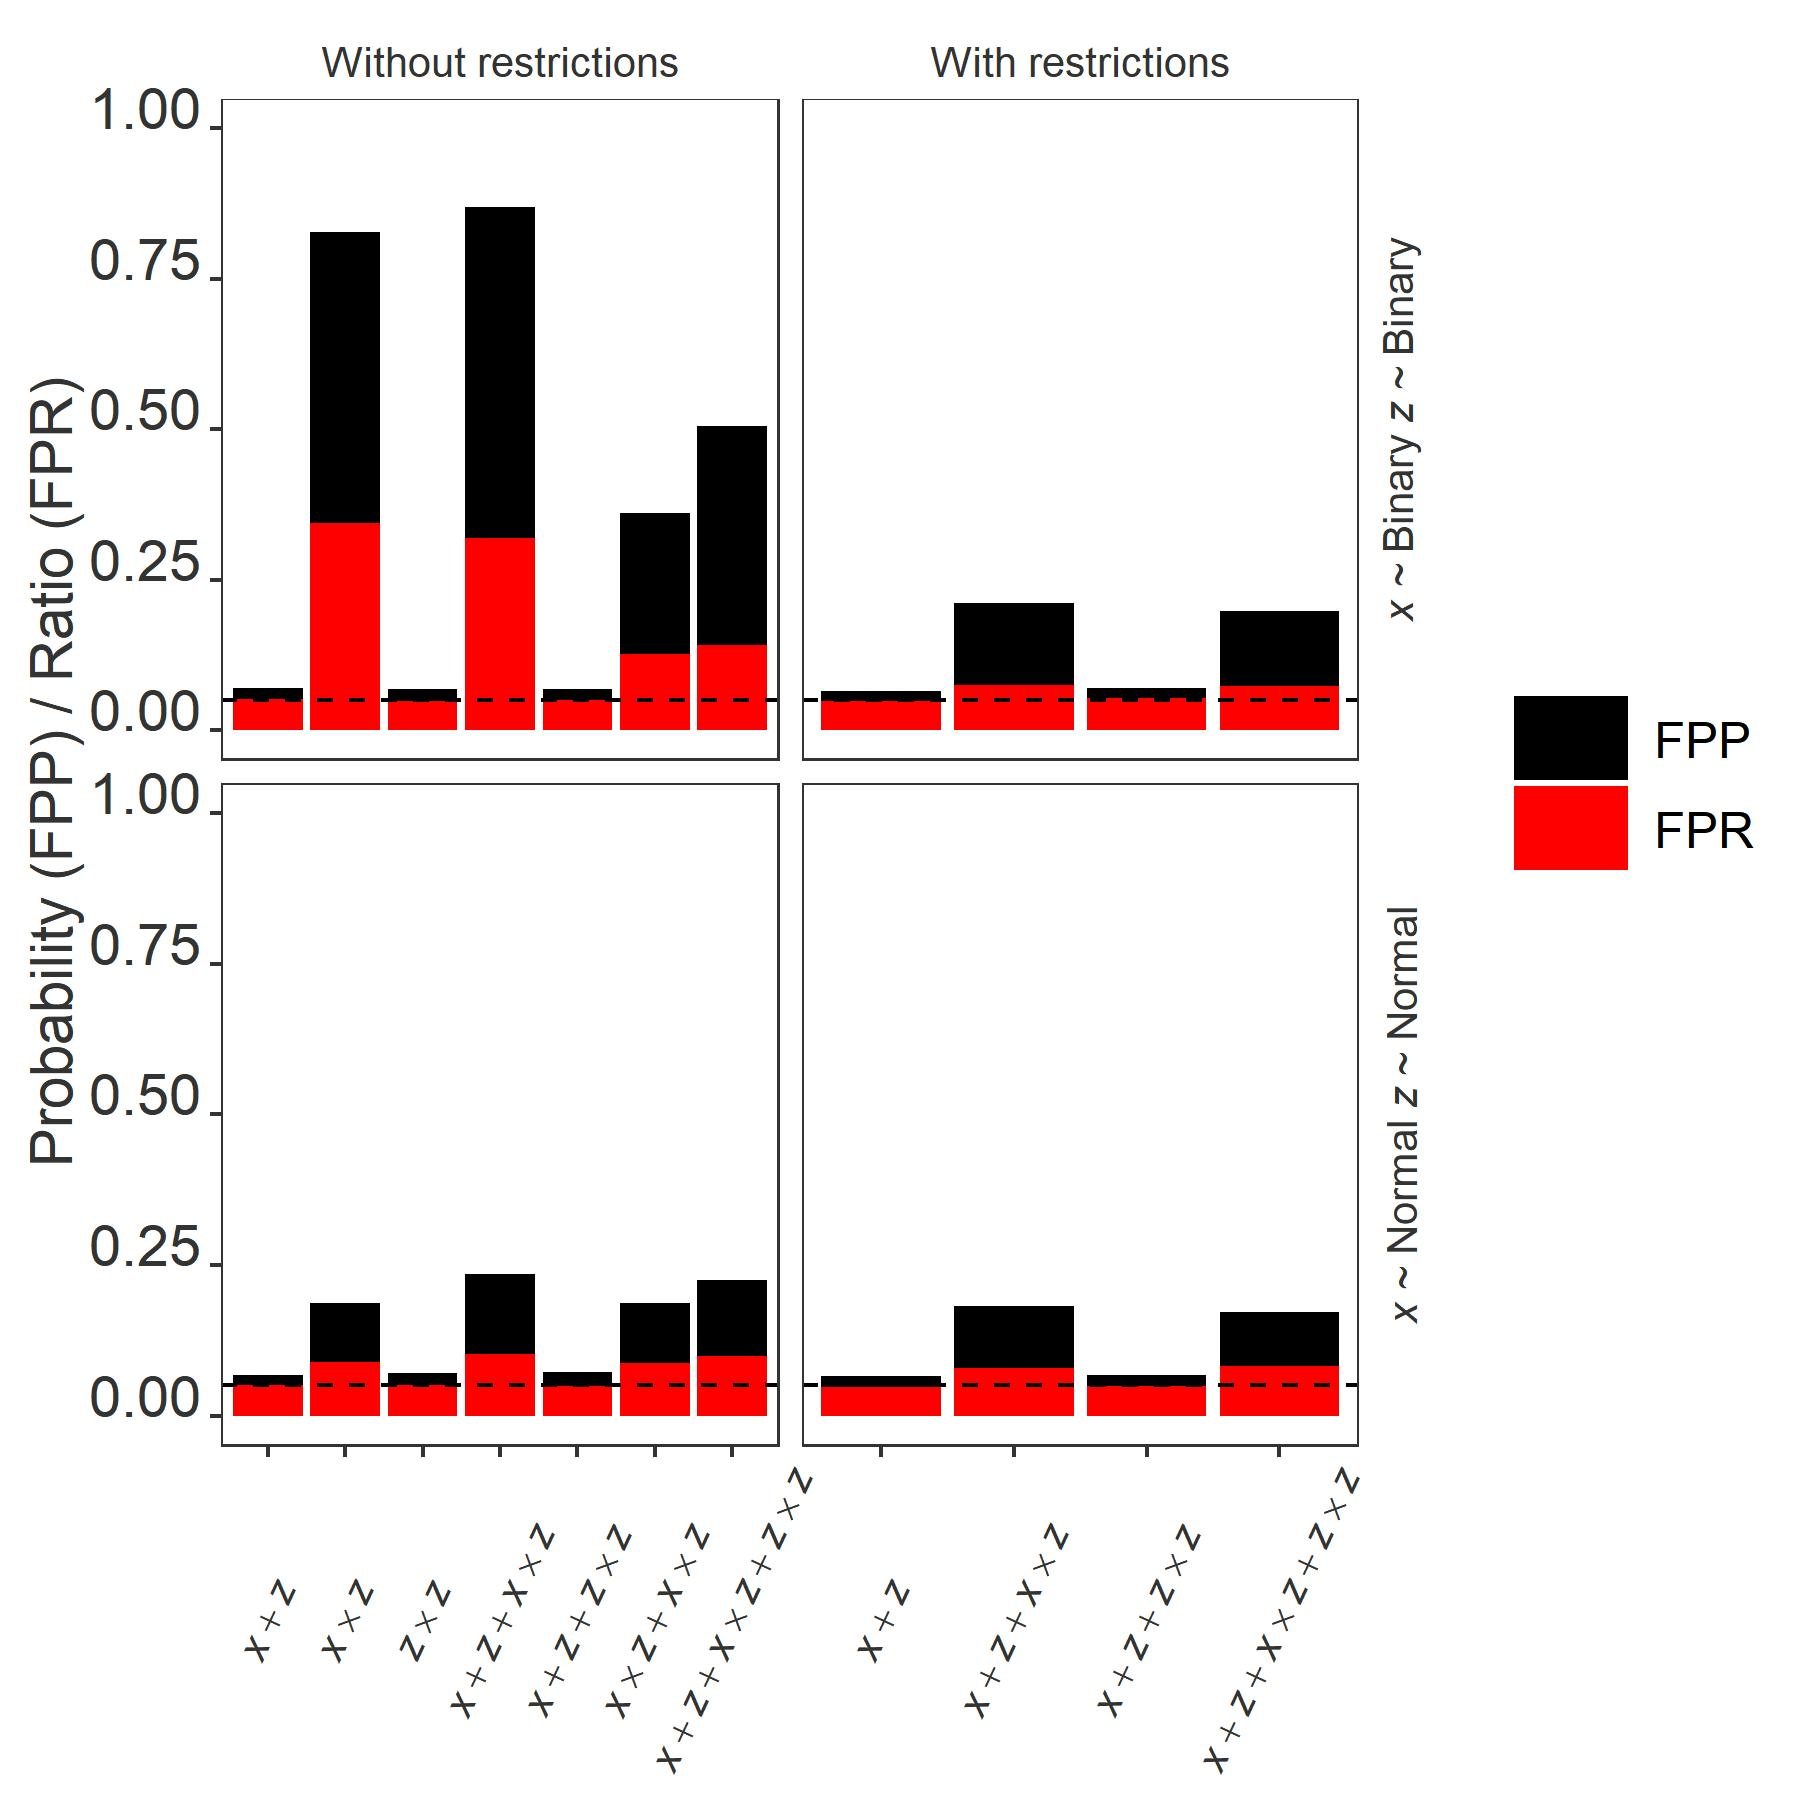
\includegraphics[width=0.6\textwidth]{R/Analysis/Result/Figures/Figure1A.jpeg}
\centering
\caption{Black is the FPP and red is FPR.  Splitting the false-positive rate by model set and whether the main effects should follow interactions or not. If Main=False we had no restrictions. Sample size set at 200, a correlation between the dependent variable and covariates set at r=0.2 and using two covariates.}
\label{fig:mainfigure}
\end{figure}

% plot of main analysis
\begin{figure}[t]
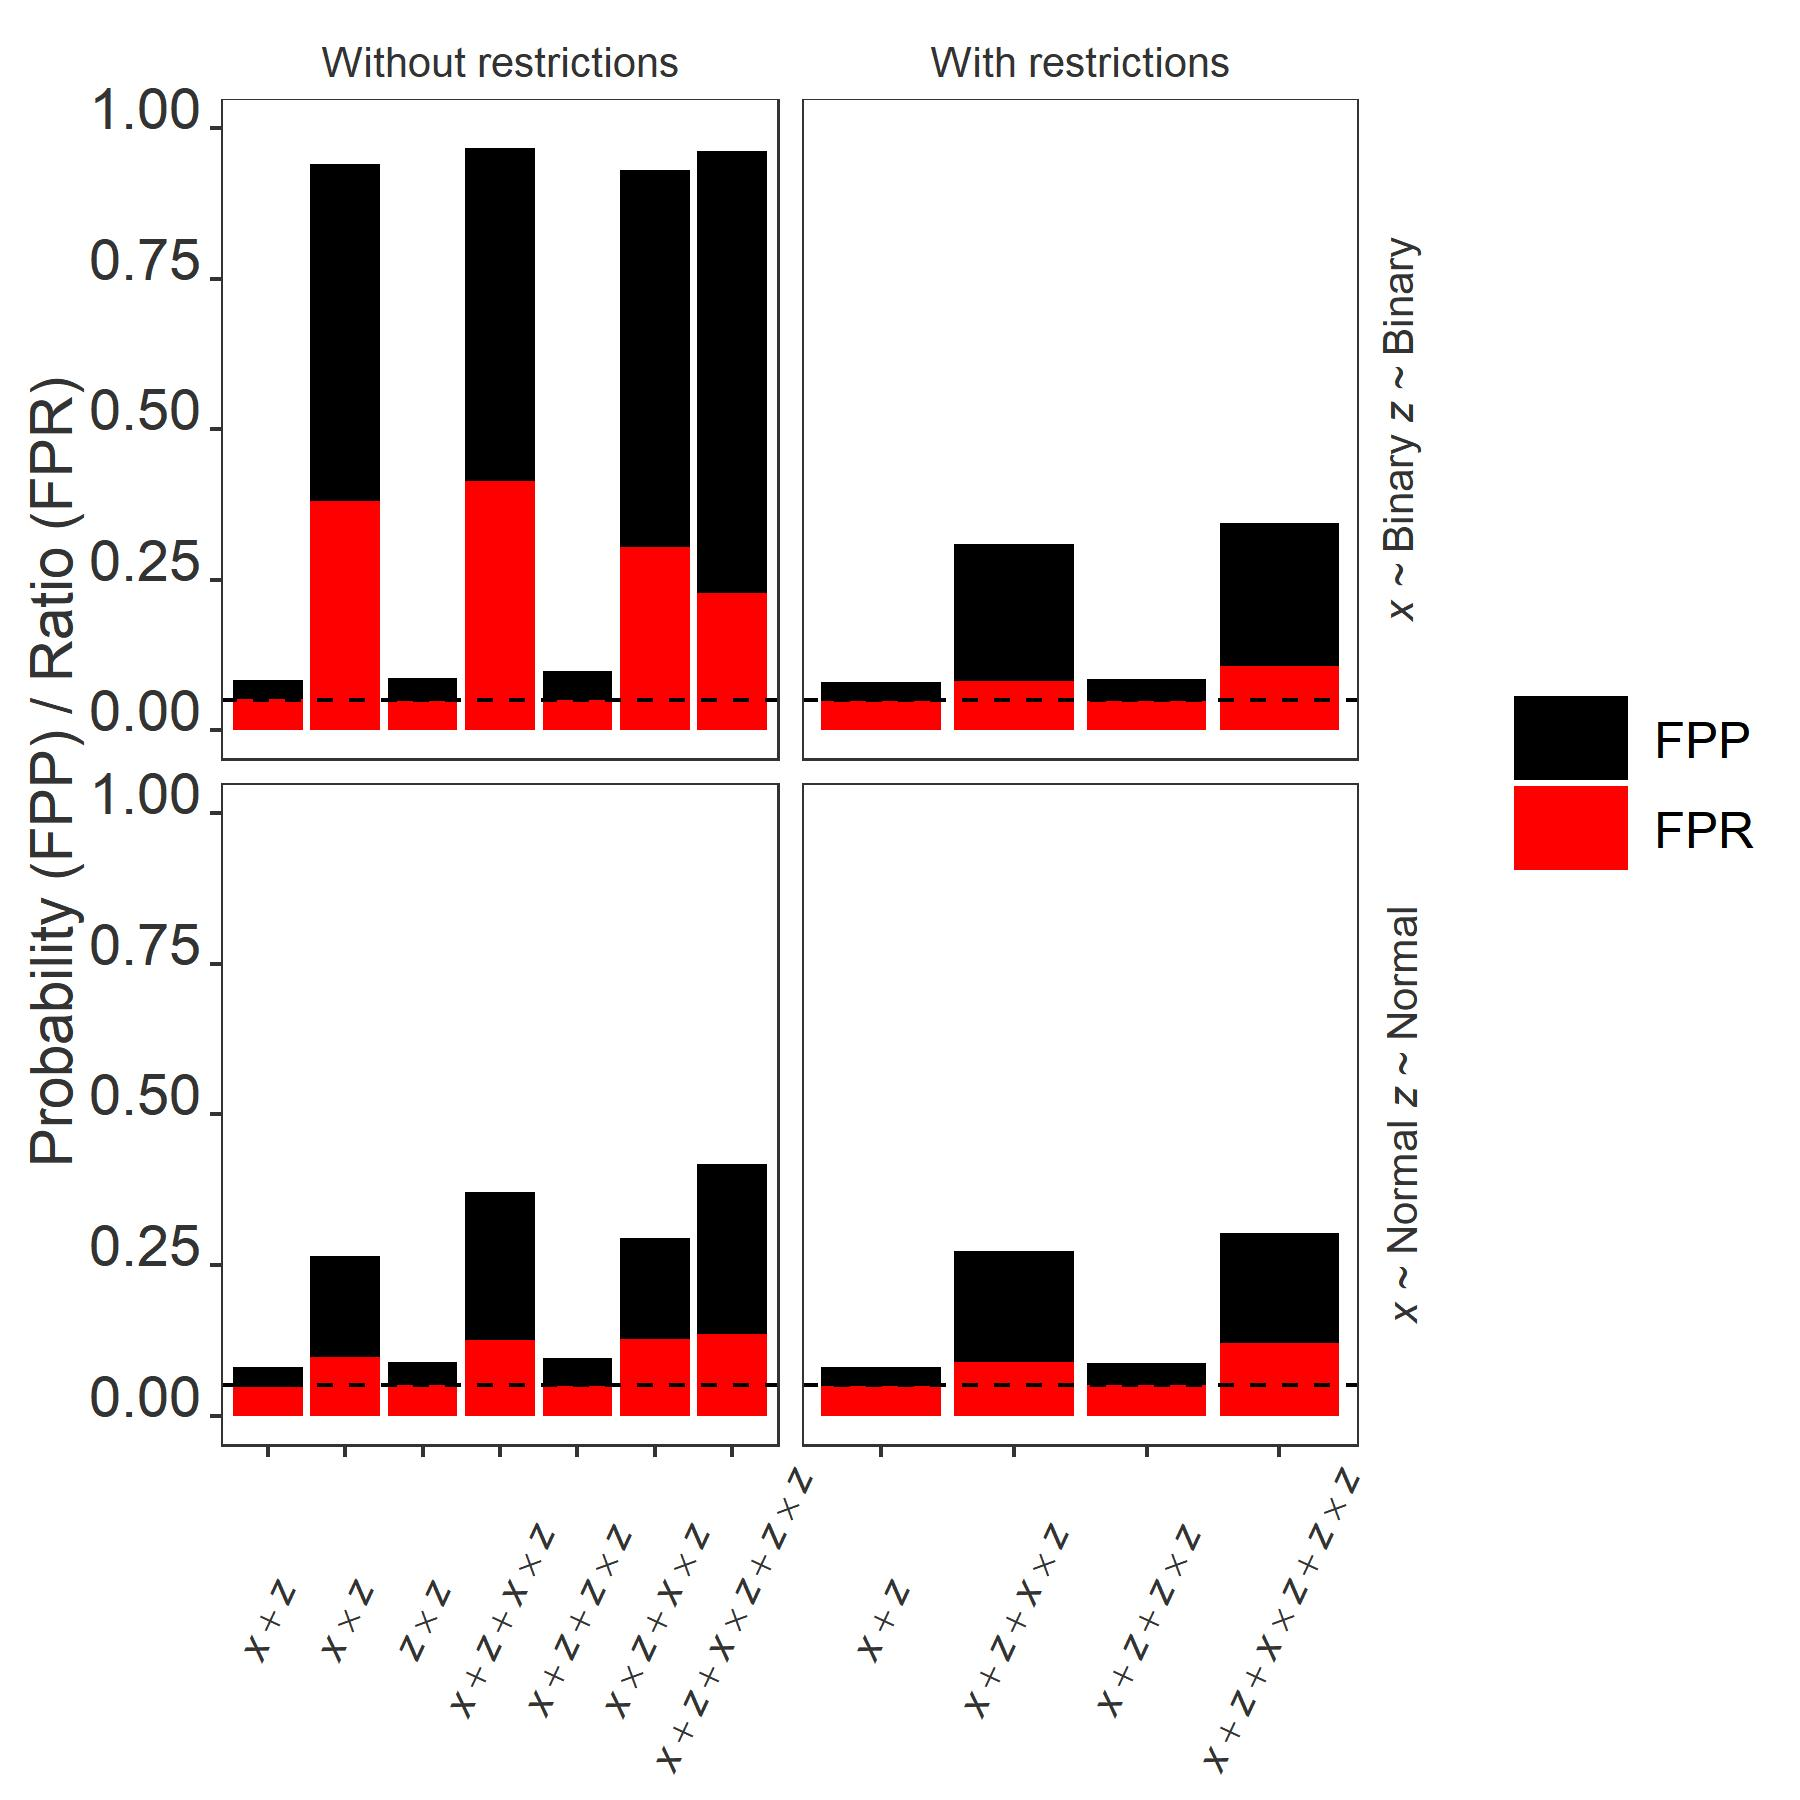
\includegraphics[width=0.6\textwidth]{R/Analysis/Result/Figures/Figure1C.jpeg}
\centering
\caption{Added effect of having one more covariate. otherwise same as Figure 1.}
\label{fig:mainfigure}
\end{figure}

\subsection{Outlier criteria}
For the outlier deletion, we were interested in how this affected across the different model sets as well. Therefore, the added effect of using the four different outlier criteria compared to not using them was plotted. Again, the sample was set to 200, and all binary variables where dummy coded. In Figure 3, the added effect of using the outlier criteria can be seen. Outlier deletion had a different added effect on the different model sets and data structures. The main contribution was within the sets where there were interactions between the covariates. Overall, the added effect to the FPP was between 4\% and 19.4\% for model sets where there was still room for an added effect. The lower added effects seen in some cases came from the fact that the FPP were already close to 100\%. This was the case for the sets where there was an interaction between the hypothesis variable and the covariates and where we allowed for models that did not have the main effect present. Using outlier criteria did not increase the FPR and in some cases deleting outliers decreased the FPR. 

\begin{figure}[t]
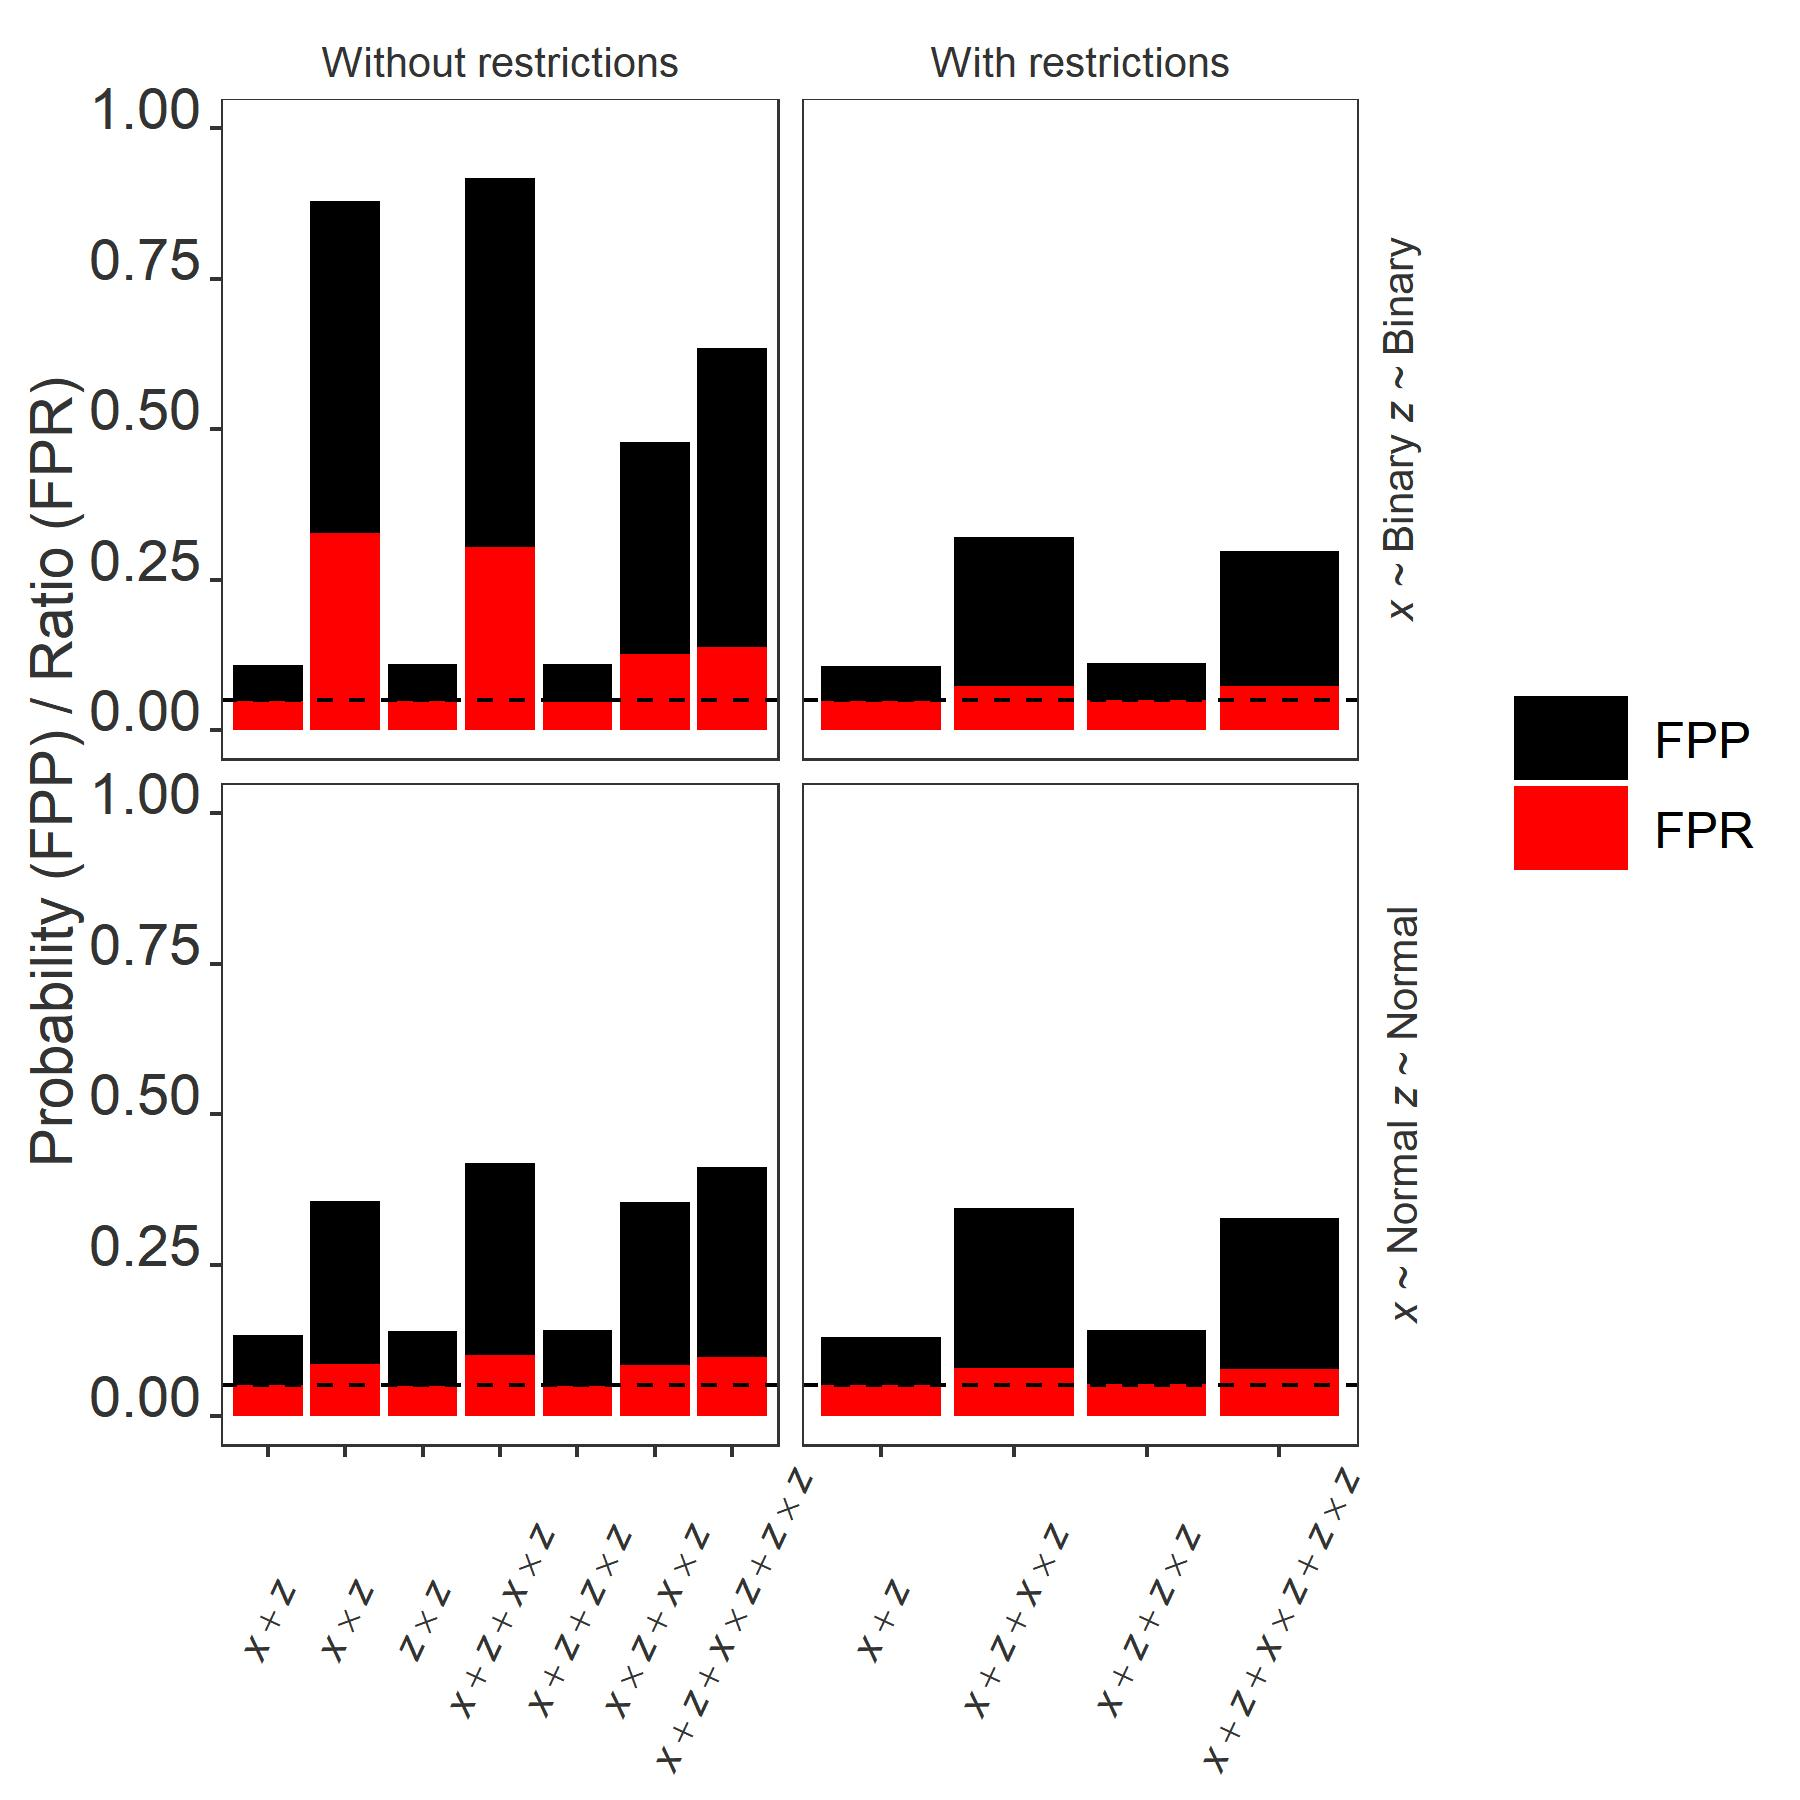
\includegraphics[width=0.6\textwidth]{R/Analysis/Result/Figures/Figure1B.jpeg}
\centering
\caption{Added effect of using multiple outlier criteria. Black is the added effect to FPP and red is the added effect to FPR.  Splitting the false-positive rate by model set and whether the main effects should follow interactions or not. If Main=False we had no restrictions. Sample size set at 200, a correlation between the dependent variable and covariates set at r=0.2 and using two covariates.}
\label{fig:mainfigure}
\end{figure}

\subsection{Multiple dependent variables}
When looking at multiple dependent variables, we again looked at the different sets of the models. We did not include outlier deletion and all binary variables were dummy coded. Collecting multiple dependent variables and using their averages increased the FPP. This was a general result overall data structures, model sets, and if main effects were included or not. The effect of using three dependent variables, and the average can be seen in Figure 3SI in supplementary information. This increase was highest for sets where there were interactions between the hypothesis variable and the covariates, no matter the data structure and other requirements. For these sets the increase in the FPP was around 15\%. The increase in the false-positive rate seems to be mainly be driven by the increase in the number of models, as the FPR did not increase for any sets. 

\subsection{Sample size and correlation}
Increasing the sample size and thereby the precision of the estimates did not seem to lower the false-positive probability. And even worse, when the constitutive terms were not included, the sample size increased the FPP (See Figure 4). In this case, the FPP went just under 100\% when the sample increased. The larger sample did not only increase the FPP, but the FPR also increased. The FPR got as high as 41\% for the set HCI with binary data and no restrictions. This means that in these sets where the FPR was 41\% just running one model from these sets would give a FPP at 41\%. 
A higher correlation between the dependent variable and the covariates also increased the false-positive rate for some sets. In general, when the correlation was higher, the FPP was higher when we did not require that the main effect followed the interactions. The sets with the highest increase were then the sets that contained HCI in some way. The effect was greatest when the data was binary and dummy coded (see Supplementary information). The increase in the FPP for these sets was between 15\% and 23\% when the correlation increased from r=0.2 to r=0.3. When the correlation increased from r=0.3 to r=0.4 it was only the sets where there was still room for a higher FPP that increased as a high number of the sets had a FPP of just below 100\% (see Figure 1SI). With this increase in the correlation also increased the FPR for the same sets. This increase was as high as 10\%. When it was required that the main effect should always be present, the FPP and FPR seemed to be stable as the correlation increased (See Figure 1SI).

\begin{figure}[t]
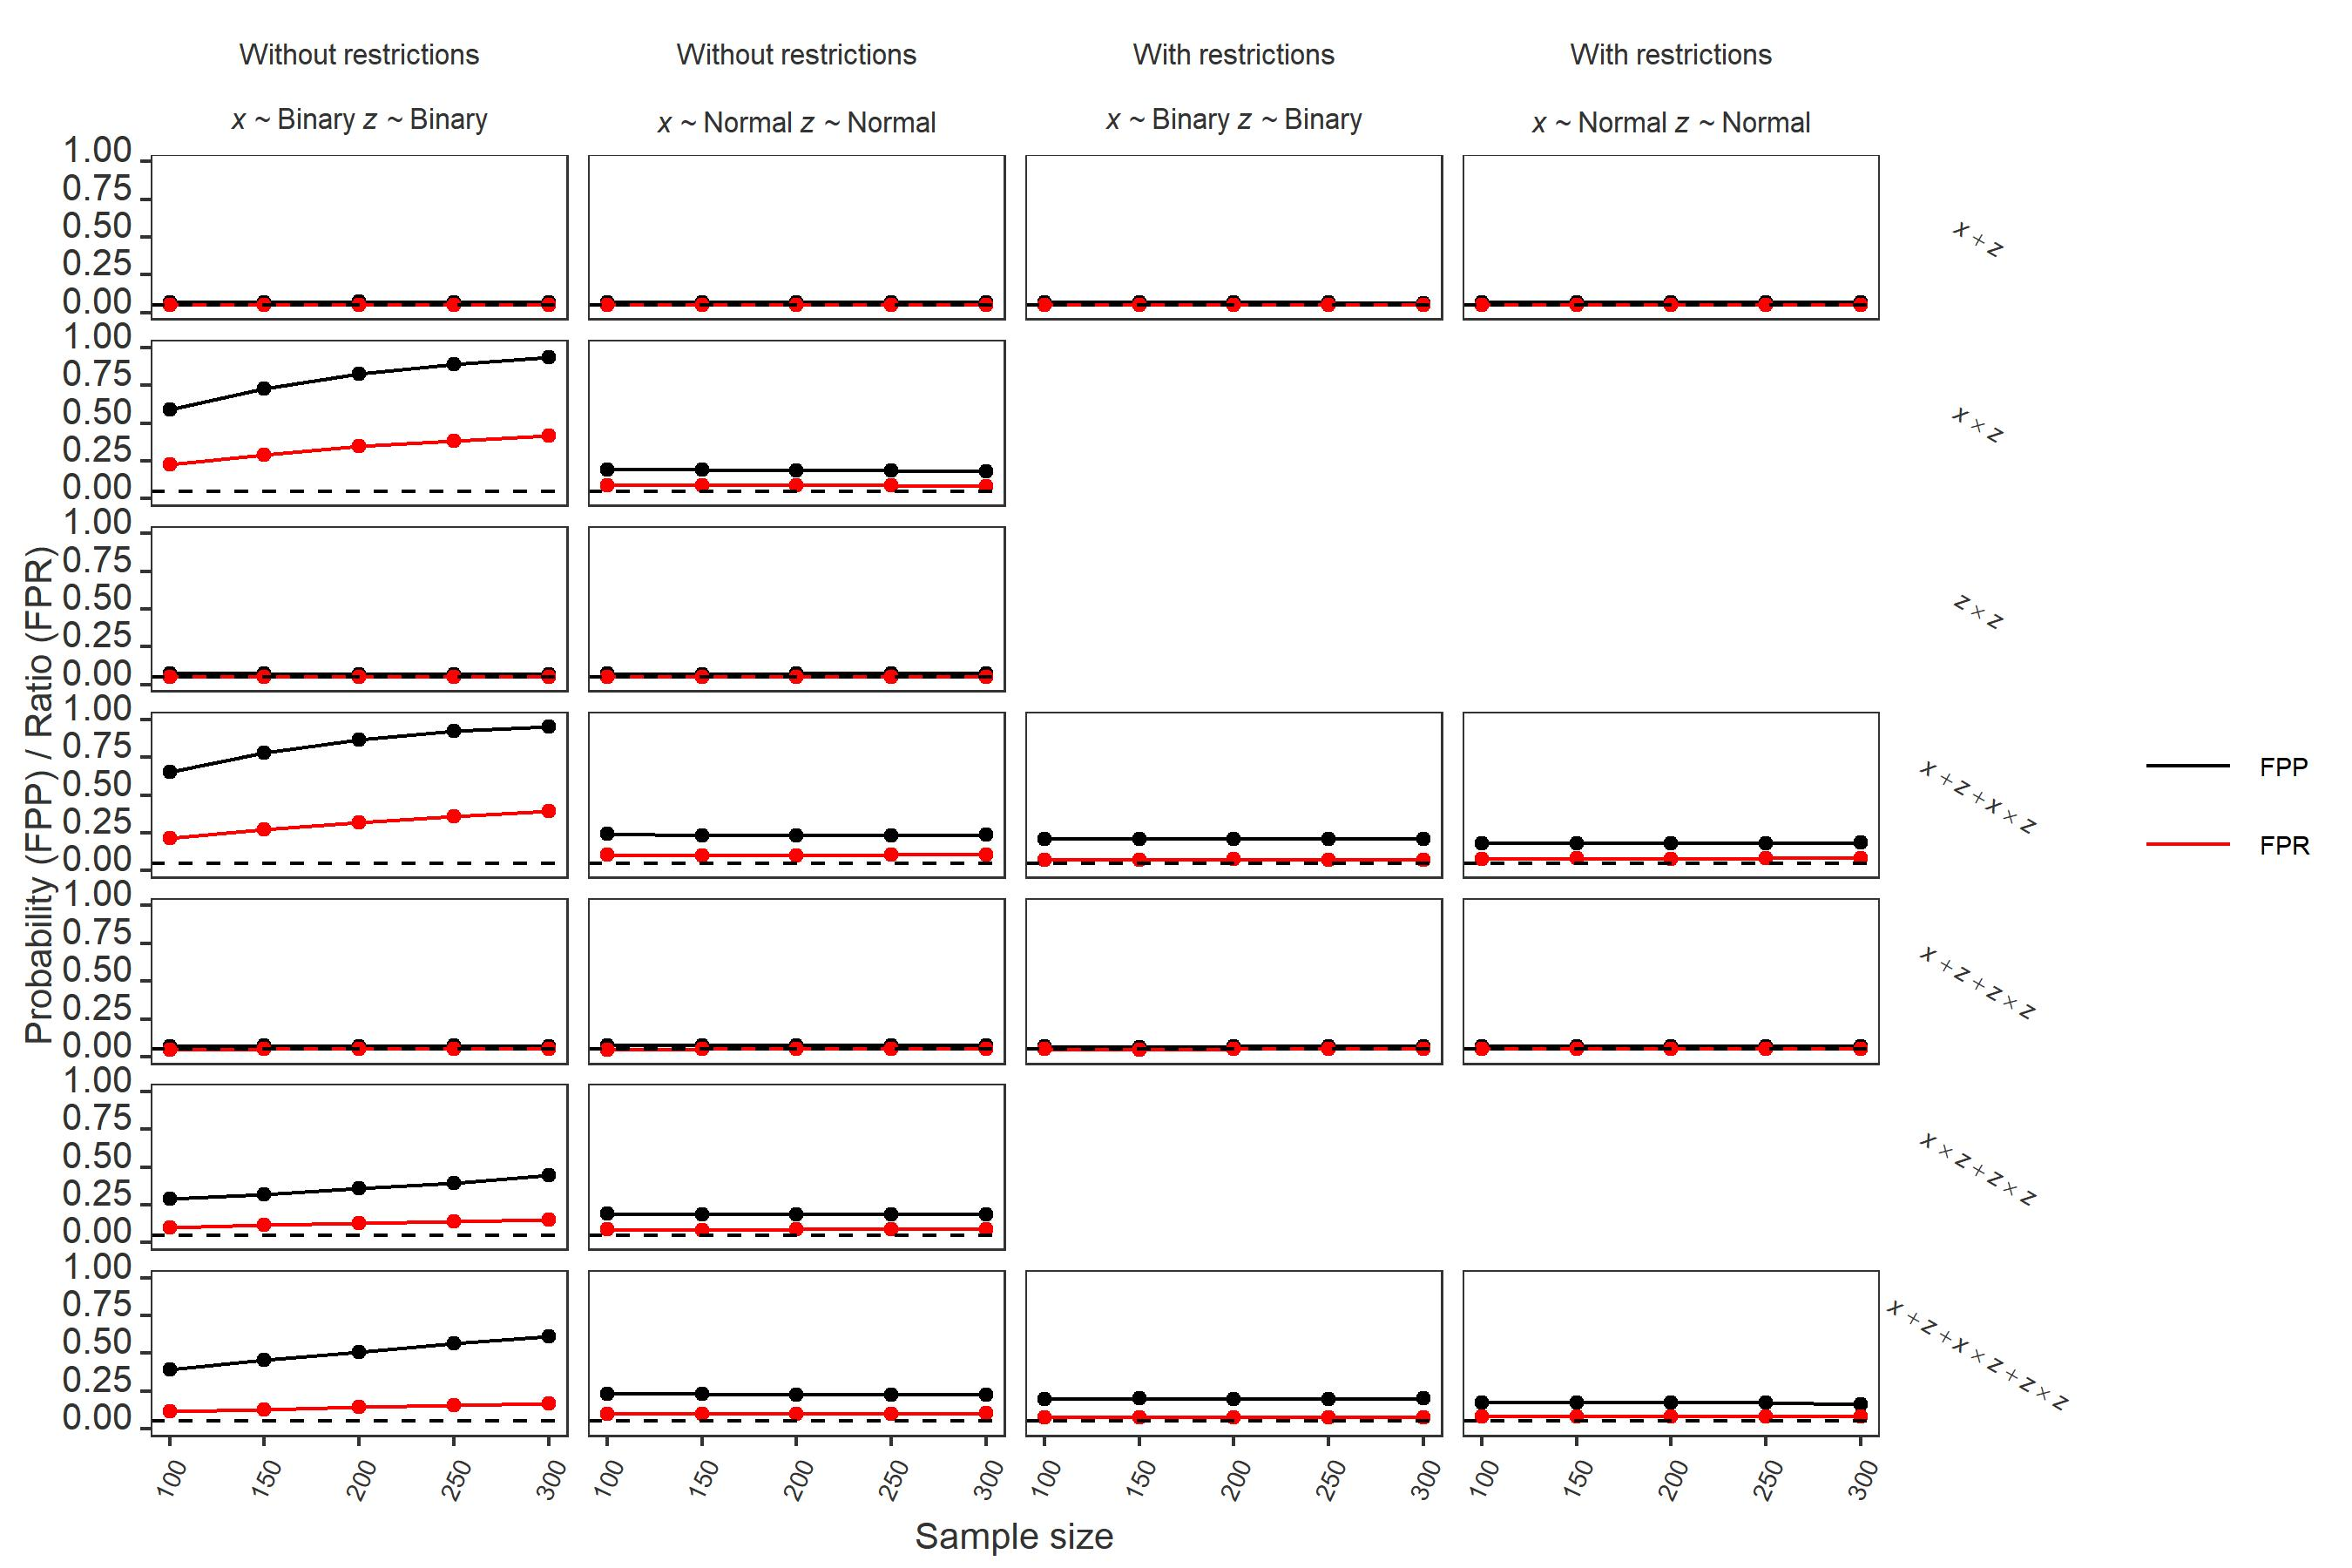
\includegraphics[width=0.6\textwidth]{R/Analysis/Result/Figures/Figure1D.jpeg}
\centering
\caption{Black is the FPP and red is FPR.  Splitting the false-positive rate by model set and whether the main effects should follow interactions or not. The effect of increasing sample size. Correlation between the dependent variable and covariates set at r=0.2 and using two covariates}
\label{fig:mainfigure}
\end{figure}
